\chapter{Project management}

\label{ch:management}
\lhead{Chapter 2. \emph{Project management}}


\nocite{Sommerville9}

%% test for site references
%\nocite{Doe:2009:Other}

This chapter describes the planning of the project.
%Section \ref{section:planning} covers project planning.
%The project schedule is detailed in section \ref{section:schedule}.
%Section \ref{section:organization} is about project organizazion.
%Quality assurace practices are described in section \ref{section:qa}
%and risk analysis is presented in section \ref{section:risk}.

\section{Project planning}
\label{section:planning}
This section describes the planning of the project including schedule, resources and tool selection.

\subsection{Project goals}

! to be merged with project objective in chapter one !

The project has various goals. One is the delivery of a report that describes all phases and relevant aspects regarding the development of the project. Another one is the development of the integration platform together with two or three prototype applications which can be used to demonstrate the functionality of the system and possibily stimulate further development of a national integration platform for eHealth.

Expected deliverables:

\begin{itemize}
\item Project report
\item Integration platform
\item Two or three prototype applications
\end{itemize}

%\subsection{Limitations}

\subsection{Project schedule}
\label{section:schedule}

\textbf{Milestones} \newline
We have identified four milestones for the project. These are associated with important events in the project lifetime and can help us to better monitor its progress. Project's milestones are shown in table \ref{table:milestones}.

\begin{table}[h]
\begin{center}
\begin{tabular}{ | l | l | l | }
  \hline
  Milestone & Date & Description \\
  \hline\noalign{\smallskip}\noalign{\smallskip}\hline
  M1 & 20.09.2013 & Basic implementation of the platform and one prototype. \\ 
  M2 & 14.10.2013 & Mid-term report delivery. \\
  M3 & 04.11.2013 & Feature freeze. \\
  M4 & 21.11.2013 & Project demonstration. Final report delivery. \\
  \hline
\end{tabular}
\end{center}
\caption{Project milestones}
\label{table:milestones}
\end{table}

\textbf{Sprints schedule} \newline
Table \ref{table:sprints} contains an overview of the Sprints in the project.
Each sprint is described in a seperate chapter.

\begin{table}[h]
\begin{center}
\begin{tabular}{ | l | l | l | }
  \hline
  Sprint & Start date & End date \\
  \hline\noalign{\smallskip}\noalign{\smallskip}\hline
  0 & 26.08.2013 & 08.09.2013 \\ 
  1 & 09.09.2013 & 22.09.2013 \\
  2 & 23.09.2013 & 06.10.2013 \\
  3 & 07.09.2013 & 20.10.2013 \\
  4 & 21.10.2013 & 04.11.2013 \\
  5 & 05.11.2013 & 21.11.2013 \\
  \hline
\end{tabular}
\end{center}
\caption{Planned sprints}
\label{table:sprints}
\end{table}

%---

\subsection{Work plan}
\label{section:workplan}

The project work plan is shown in figure \ref{figure:work-splan}.

\newpage
\begin{landscape}
\begin{figure}[h]
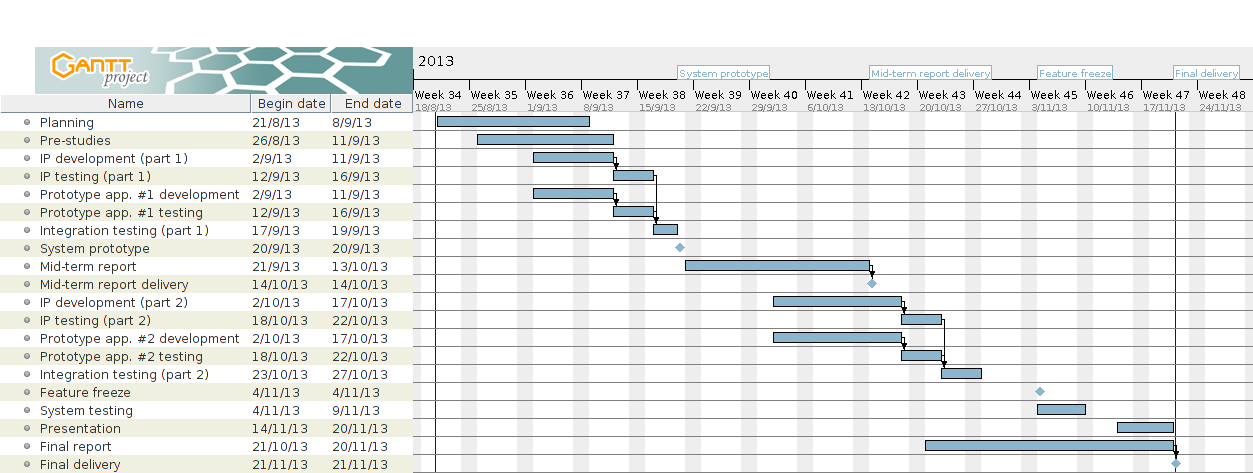
\includegraphics[scale=0.66]{../Figures/gantt-diagram.png}
\caption{Gantt diagram}
\label{figure:work-splan}
\end{figure}
\end{landscape}

%---

\subsection{Resources}
\label{section:resources}
The team consists of three members from different educational backgrounds and with different skills.
In order to better distribute the work among us, we have created a skill matrix regarding the technologies involved in the project.
The skills are valued on a scale of zero to five based on criterias detailed in table \ref{table:skillscale}.
Each value corresponds to a certain degree of proficiency, as described in table \ref{table:proficiency}.
The skill matrix is shown in table \ref{table:skillmatrix}.

\begin{table}[h]
\begin{center}
\begin{tabular}{ | c | l | l | }
  \hline
  Level & Proficiency & Criteria \\
  \hline\noalign{\smallskip}\noalign{\smallskip}\hline
  0 & None		& Has no clue what we're talking about. \\
  1 & Basic		& Has read about it.\\
  2 & Fair		& Has studied it at school.\\
  3 & Good		& Personal interest, use in small-medium sized projects.\\
  4 & Very good	& Strong personal interest, use in medium-large sized projects. \\
  5 & Excellent	& 10+ Years of work experience. \\
  \hline
\end{tabular}
\end{center}
\caption{Skill's scale explanation}
\label{table:skillscale}
\end{table}

\begin{table}[h]
\begin{center}
\begin{tabular}{ | c | l | l | }
  \hline
  Level & Proficiency & Description \\
  \hline\noalign{\smallskip}\noalign{\smallskip}\hline
  0 & None		  & Cannot perform the task \\
  1 & Basic     & Can perform the task with some help from other people \\
  2 & Fair		  & Can perform the task almost indipendently \\
  3 & Good		  & Can perform the task without any help \\
  4 & Very good	& Can help others to complete the task \\
  5 & Excellent	& Can help others to complete the task \\
  \hline
\end{tabular}
\end{center}
\caption{Proficiency level description}
\label{table:proficiency}
\end{table}

\begin{table}[h]
\begin{center}
\begin{tabular}{ | l | c | c | c | c | c | c | c | c | }
  \hline
  Team member & Java & JS & Android & Database & CSS & jQuery & Spring & LaTeX \\
  \hline\noalign{\smallskip}\noalign{\smallskip}\hline
  Anders & 4 & 4 & 3 & 4 & 4 & 2 & 3 & 1 \\
  Emanuele & 4 & 1 & 3 & 2 & 1 & 1 & 0 & 3 \\
  Sebastian & 4 & 4 & 2 & 4 & 3 & 4 & 0 & 3 \\
  \hline
\end{tabular}
\end{center}
\caption{Skill matrix}
\label{table:skillmatrix}
\end{table}


%---

\subsection{Project tools}
\label{section:tools}
This section describes the different tools used throught the project.

\begin{description}

\item[Git and GitHub]
Git is one of the most used version control systems. Although it is mostly used for code, it can be used to manage other types of file such as LaTeX. GitHub is a repository hosting service for Git projects which offers a web-based fronted. We have decided to use Git because of the familiarity we had with it. We used Git for managing both the code and the report.

\item[Scrumdo]
Scrumdo is a web-based Scrum tool. It has many features such as a Scrum board, stories and iteration management
as well as time-tracking. It is possibile to export the data on Scrumdo to other formats such as Excel tables.
Although most of the features are free to use, some of them require a membership. We managed to obtain
time-limited membership for free after writing to the people running the service. Scrumdo proved an useful tool
for our project. We used Scrumdo to populate our product and sprint backlogs, size stories, track assignees
and times, burnout charts.

\item[Sublime Text]
Sublime Text is a popular, cross-platform editor which offers advanced features.
We used Sublime Text for editing the report and for coding JavaScript, CSS.

\item[IntelliJ IDEA]
A popular, feature-rich Java IDE. We used it to develop Android applications and for Spring coding.

\item[Apache Maven]
Maven is an open and cross-platform build system for Java projects which, among other things, takes care of dependecies. Maven is powerful and well documented and seemed an optimal choice for our project also because of the familiarity we had with it.

\item[LaTeX suite]
LaTeX is a powerful language used to prepare documents which is widely used in academical environments. LaTeX takes care of the formatting of the document allowing the writer to focus on the contents, moreover LaTeX documents can be written with any text editor and then compiled to PDF documents. We chose LaTeX because of its advanced features and the familiarity we had with it.

\item[Google Drive and Google Docs]
Google Drive is a service which lets you access your files from everywhere and share them with other people. It is tightly integrated with Google Docs, a web-based productivity suite. We used Google Drive to share documents within the team and with the customer and supervisor.
Many of the documents and diagrams produced for the project were created using Google Docs.

\item[Violet UML]
A free, Java (cross-platform) UML editor. Violet UML was used for producing use cases and sequence diagrams.

\item[GanttProject]
A free, Java (cross-platform) tool for generating Gantt diagrams. We used it to produce a diagram of the work plan.

\item[Skype]
A popular instant-messaging client that also supports audio and video communication.
Skype was used throught the project to keep in touch with the customer and team members.

\item[Facebook]
Facebook is a social networking service. The team created a group on Facebook that was used as a bulleting board for internal communications.

\item[Travis CI]
Travis CI is an automated build service...
% we should write two more lines here.

%Balsamiq Mockups looks great, it would be cool to do some mockup with this!!
%Lucidchart maybe we can opt for a free solution like violet UML.

\end{description}


%\subsection{Version control procedures}


%---

\section{Project organization}
\label{section:organization}

This section describes the organizational aspects of the project such as roles description and allocation, meetings schedule and
specific group dynamics.

\subsection{Role description}
We have identified a number of roles in this project. Although each role has different, distinct responsabilities, we see all roles as equally important for the success of this project.

\begin{description}
\item[Project manager]
%supposedly, there is no project manager in scrum !!
The project manager has the responsability of managing the project.
This includes people management, high level project planning and risk analysis.
The project manager is also responsible of producing weekly status reports and communication with the customer and supervisor.
\item[Scrum master]
The scrum master has the responsability of helping team members perform Scrum.
\item[Product owner]
The product owner is responsible of approving and prioritizing the product
requirements in order to steer its development in the direction he sees fit.
%\item[System architect]
\item[Secretary]
Responsible for taking notes during meetins and booking rooms.
\item[Quality assurance]
Ensures that quality practices are in place and use.
\item[Web developer]
Responsible for web development. Oversees and takes initiative on web development (front-end).
\item[Droid developer]
Responsible for Android development. Oversees and takes initiative on Android applications development.
\item[System developer]
Responsible for developing the Spring backend, including database coding. Takes care of system deployment.
\end{description}

\subsection{Role allocation}

\begin{figure}[H]
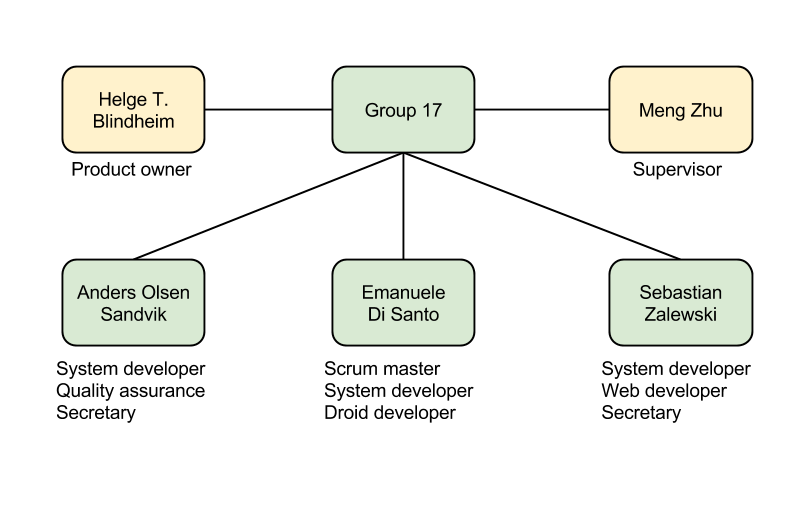
\includegraphics[scale=0.5]{../Figures/organizational-diagram.png}
\caption{Organizational diagram}
\label{figure:orgdia}
\end{figure}

Roles were allocated primarily on team members' competences.
Those roles that were left unassigned were taken up by members who volunteered for them upon approval 
of other team members.
Because we were only three people, all of us had more than one role. Sometimes, roles were shared.
We tried to balance roles evenly between ourselves and achieve a flat group organization where no member
had a prominent role on others. Table \ref{table:roles} shows roles allocation within the group.
See \ref{figure:orgdia} for an diagram of how the group is organized.

\begin{table}[h]
\begin{center}
\begin{tabular}{ | l | l | }
  \hline
  \textbf{Member} & \textbf{Roles} \\
  \hline\noalign{\smallskip}\noalign{\smallskip}\hline
  Anders Olsen Sandvik  &  System developer, Secretary, Quality assurance\\
  Emanuele Di Santo     &  Project manager, Droid developer, System developer\\
  Sebastian Zalewski    &  Web developer, System developer, Secretary\\
  \hline
\end{tabular}
\end{center}
\caption{Members' roles}
\label{table:roles}
\end{table}

\subsection{Weekly meeting schedule}
During the early stages of the project the team has agreed on a meeting schedule.

\begin{description}

\item[Monday] (from 10 to 19 - 9 hours total) \\
\textbf{[10.00 - 11.00] Weekly startup meeting}\newline
At the begin of each week we would review the progress done during the previous and discuss the plan for the next.
We also discussed any problems encountered.
This internal meeting would follow the last Status Report document.
\newline\textbf{[11.00 to 12.00] Customer meeting}\newline
During the meeting with customer we would discuss with him the work done and share our plan for the next week.
This was done in order to help us prioritize our work to better suit the customer's interest.
\newline\textbf{[12.00 to 13.00] Supervisor meeting}\newline
The group would go through the status report and bring up issues or problems with the project.
We tried to give the supervisor the best understanding possible of our project especially regarding
its progress and group dynamics.
\newline\textbf{[13.00 to 14.00] Lunch}\newline
The group had lunch together on Mondays. It is good to eat together and chat about things other than the project.
It helps getting to know each other better.
\newline\textbf{[14.00 to 19.00] Collective work session}

\item[Wednesday] (from 15 to 19 - 4 hours total) \\
\textbf{[15.00 to 19.00] Collective work session}
\end{description}

\subsection{Group dynamics}
\label{section:dynamics}

Group dynamics are probably the most critical aspect of this project.
%The people involved in this project, and in particular its group members are the most critical asset of the project itself.
It would be safe to say that due to the nature of the project itself, its success is based primarily on group dynamics.
We are, in fact, a group of people working to deliver a product to another group of people.
It is easy to convince ourselves that in this case (and many other) people management is essential for the product to be successful.
Any successful software project relies on successful group dynamics because no project can be accomplished by a single man.
We understand that the role of a good project manager is basically people management.
This encompasses a set of practices, precautions and knowledge which we have taken into consideration and tried our
best to make our own.

\begin{description}

\item[Understand people]
This is of course a fundamental prerequisite of people management: there can be no people management without some kind of understanding.

\item[Lead by Example]
A project manager should lead other team members by giving them a good example: being enthusiastic about his job
and doing it with a positive attitude.

\item[Communicate]
It's important to give everybody a \'big picture\'.

\item[Motivate]
A team's commitment will greatly improve many variables in a software project.
People are inevitably influenced by other people around them, especially when they work together.
If any member has a low commitment to the project his attitude will influence negatively other team members.

A good project manager will motivate the team to work well and gratify members who do so.
It is a duty of the project manager to instill a positive and enthusiastic attitude in the team.

To achieve this task, it is important to identify personality types among a group so that
motivation can be more effective. These can be divided into three categories:
  \begin{itemize}
  \item Self-oriented: the work has the purpose to achieve personal interestes.
  \item Task-oriented: the motivation is related to the task itself.
  \item Interaction-oriented: the motivation is related to social interaction.
  \end{itemize}

It is desiderable that within a group such personality types are balanced.

In our case, the project manager tried motivating the group by rewarding good jobs
and outlining the importance of the project itself as a chance to acquire knowledge,
to get a good grade (academic achievement) and to do something that stimulated further
research and work in the field.

\item[Cooperation]
People should be encouraged to work together, share ideas and thoughts.
We should avoid having one team member whose role is predominant on others'.

During meetings, both internal and external, we had one team member
act as a \'meeting leader\', guiding the customer, supervisor or other team members through
the meeting agenda. However, the project manager made sure to involve all team members
in the conversation, asking their opinion on the current topic being discussed
or in order to let them explain their what they did and how.
When the supervisor or the customer asked questions, he made sure not to be the only one
answering by inviting other team members to do so.

\item[Size matters]
The fact that the group is made of three members definitely plays a factor in group dynamics
and in projet management. Though many may see it as a weakness or downside of a group we believe
in our case it was not, or rather it proved more a strenght than a weakness.
In software development, just like in any other engineering practice assigning many people
at a task is unlikely to produce better results than a sufficiently small but motivated group.
%Just like it takes one month to ferment wine, no matter how many people are involved.
Although having a small team means that flexibility in group composition is absent and
the technical skill pool is reduced it is important to realize that a small team
can be more easily motivated and achieve a higher degree of cooperation.
To do so, care should be taken into not letting any member of the group become
a \'black sheep\'. Team members should respect each others and their respective work,
nobody should feel less important or cut out of the decision making process.

\item[Distance matters]
During the project one team member moved to Oslo and got a full-time job.
This important event required some adjustment to project management strategy.

....



\end{description}


%pregnant woman mistake

%flexibility in group composition is absent.
%technical skill pool is reduced.

%possibility of better cooperation
%easily motivated

%black sheep


\section{Quality assurance}
\label{section:qa}

This section describes what practices we put in use to ensure the quality of the product and the report.


\subsection{Quality of the documentation}
Each document should be reviewed by another person other than the writer.
Especially for the report, we took care of reviewing each other's work in order to ensure
consistency and correctness throughout the document.

\subsection{Templates}
We have established templates for the following:
\begin{enumerate}
\item status reports
\item meeting notes for all meetings
\item meeting agendas for supervisor meetings
\end{enumerate}

Templates can be found in appendix \ref{AppendixC}.

\subsection{Standards}

\textbf{Coding style}
The adopted a camelcase notation  for function and variables in Java

database, comments, function, brackets..

\textbf{File naming}


\subsection{Status report}
As requested, the group submitted a document called 'status report' on a weekly basis.
The document contained a summary of the all progress made on the project during the week.
This included what the group had been working on, milestone achieved, meetings summary, eventual problems\ldots
%The status report would be sent to the supervisor on Sundays to be discussed on Mondays.

\subsection{Internal meetings}
After one group member moved permantly to Oslo, we scheduled internal meetings to be held on Skype
on a weekly basis. The secretary took notes during the meetings, which were then stored on Google Drive.

\subsection{Customer meetings}
Customer meetings were held on a weekly basis (on Mondays) at ten o'clock.
Because the customer was in different city, meetings were held on Skype.
The secretary would take notes for the meeting which would then be stored on Google Drive,
where the customer could easily access them.
%to which the customer had access.
% based on templates found in \ref{AppendixC}.
%At the end of each meeting, we would agree with the customer about the time of our next meeting.
Notably, we didn't have meeting agendas for customer meetings because we esplicitely agreed
on the time of our next meeting and implicitely on the topics to be discussed.
%agreed on the topics to be discussed next time during our meeting.

\subsection{Supervisor meetings}
Supervisor meetings were held on a weekly basis.%, on Mondays.
Their purpose was to give our supervisor a good overview of how we were carrying out the process
and ensure that we weren't missing any important details
The secretary was responsible of taking notes during the meeting.
These would be attached to our status report and meeting agenda and sent to the supervisor
for approval.
Each meeting we would go through the status report which had been submitted during the week-end
and 


\newpage
\section{Risk management}
\label{section:risk}

Risk analysis is an important activity in any engineering process.
Any project has inherently some risks of which it's important to have a clear
understanding about so that mitigation and remedy strategies can be prepared
and put in use before it's too late. We have kept our risk analysis updated on a weekly
basis when possibile and made it available both to the customer and the supervisor through
Google Drive for feedback.

See table \ref{table:likelihood} and \ref{table:impact} for a textual description of
likelihood and impact levels respectively. See table \ref{table:risks} for risk analysis.

\begin{table}[h]
\begin{tabular}{ | l | p{11.5cm} | }
  \hline
  \textbf{Likelihood} & \textbf{Description} \\
  \hline\noalign{\smallskip}\noalign{\smallskip}\hline
  Low       & It is unlikely the factor will show up. \\
  Moderate  & There is a moderate chance the factor will show up. The risk should be monitored. \\
  High      & The risk factor is very likely to happen. The risk should be constantly monitored. \\
  \hline
\end{tabular}
\caption{Likelihood values description}
\label{table:likelihood}
\end{table}

\begin{table}[h]
\begin{tabular}{ | l | p{11.5cm} | }
  \hline
  \textbf{Impact} & \textbf{Description} \\
  \hline\noalign{\smallskip}\noalign{\smallskip}\hline
  Low       & The risk will have a minor impact which won't hinder the success of project. \\
  Moderate  & The risk will have a moderate impact. It should mitigated. \\
  High      & The risk can possibily have very negative consquences. Mitigate constantly. Have a remedy strategy ready. \\
  \hline
\end{tabular}
\caption{Impact values description}
\label{table:impact}
\end{table}

\newpage

\begin{table}[h]
\begin{tabular}{ | l | p{11.5cm} | }

  \hline
  Risk ID & \textbf{1} \\
  \hline\noalign{\smallskip}\noalign{\smallskip}\hline
  Risk Factor   & \textbf{Internal conflicts} \\
  Consequences  & Stress, decrease in member’s commitment to group work.\\
  Likelihood    & Low \\
  Impact        & Moderate \\
  Mitigation    & Communication is the key. Get to know each other. \\
  Remedy        & Try to solve the problem democratically. \newline
                If that fails the project manager should be fair but firm in his actions. \\
  \hline
  
  \hline\noalign{\smallskip}\noalign{\smallskip}\hline
  Risk ID & \textbf{2} \\
  \hline\noalign{\smallskip}\noalign{\smallskip}\hline
  Risk factor   & \textbf{Change of requirements} \\
  Consequences  & Slow progress, planning problems. Failure to meet requirements \\
  Likelihood    & Moderate \\
  Impact        & Moderate \\
  Mitigation    & Agree on project scope’s and an initial set of core, high level requirements with the customer early on. \\
  Remedy        & Prioritize tasks and reschedule work accordingly. \\
  \hline

  \hline\noalign{\smallskip}\noalign{\smallskip}\hline
  Risk ID & \textbf{3} \\
  \hline\noalign{\smallskip}\noalign{\smallskip}\hline
  Risk factor   & \textbf{Poor project planning} \\
  Consequences  & Failure to meet deadlines. Bad grades !\\
  Likelihood    & Moderate \\
  Impact        & High \\
  Mitigation    & Produce and keep updated the necessary documents.
                Share planning details with the team and the supervisor for feedback. \\
  Remedy        & The team should reflect on what has gone wrong during the last iteration and
                share their thoughts on how to improve planning. \\
  \hline

  \hline\noalign{\smallskip}\noalign{\smallskip}\hline
  Risk ID & \textbf{4} \\
  \hline\noalign{\smallskip}\noalign{\smallskip}\hline
  Risk factor   & \textbf{Underestimation of project workload} \\
  Consequences  & Slow progress, failure to meet deadlines.Excessive workload at the end of the semester. \\
  Likelihood    & Moderate \\
  Impact        & High \\
  Mitigation    & Good planning and pre-studies on technologies involved. \\
  Remedy        & Try to prioritize tasks. Assign tasks to the right people (maybe using a skill matrix) and motivate them. \\
  \hline

  \hline\noalign{\smallskip}\noalign{\smallskip}\hline
  Risk ID & \textbf{5} \\
  \hline\noalign{\smallskip}\noalign{\smallskip}\hline
  Risk factor   & \textbf{Implementation problems} \\
  Consequences  & Delays, failure to meet requirements. \\
  Likelihood    & Low \\
  Impact        & Moderate \\
  Mitigation    & Thorough pre-studies. Avoid using complicated technologies. \\
  Remedy        & Assign tasks to the right people (maybe using a skill matrix) and motivate them. \\
  \hline

\end{tabular}
\caption{Risk analysis}
\label{table:risks}
\end{table}

\begin{table}[h]
\begin{tabular}{ | l | p{11.5cm} | }
  \hline

  Risk ID & \textbf{6} \\
  \hline\noalign{\smallskip}\noalign{\smallskip}\hline
  Risk factor   & \textbf{Data loss} \\
  Consequences  & Missing deliverables. Failure to meet deadlines. \\
  Likelihood    & Low \\
  Impact        & High \\
  Mitigation    & Schedule regular backups. \\
  Remedy        & Recover the most recent backup. \\
  \hline

  \hline\noalign{\smallskip}\noalign{\smallskip}\hline
  Risk ID & \textbf{7} \\
  \hline\noalign{\smallskip}\noalign{\smallskip}\hline
  Risk factor   & \textbf{Illness} \\
  Consequences  & Slow progress. \\
  Likelihood    & Moderate \\
  Impact        & Moderate \\
  Mitigation    & Proper clothing, common sense.. \\
  Remedy        & If the illness is prolonged, work needs to be rescheduled accordingly. \\
  \hline

  \hline\noalign{\smallskip}\noalign{\smallskip}\hline
  Risk ID & \textbf{8} \\
  \hline\noalign{\smallskip}\noalign{\smallskip}\hline
  Risk factor   & \textbf{Internal communication problems} \\
  Consequences  & Slow progress, excessive workload for some members. \\
  Likelihood    & Moderate \\
  Impact        & Moderate \\
  Mitigation    & Schedule regular Skype calls. \\
  Remedy        & Take notes for each meeting and have them approved by the team. \\
  \hline

  \hline\noalign{\smallskip}\noalign{\smallskip}\hline
  Risk ID & \textbf{9} \\
  \hline\noalign{\smallskip}\noalign{\smallskip}\hline
  Risk factor   & \textbf{Study of HealthVault takes too long} \\
  Consequences  & Delays in report work and overall system development. \\
  Likelihood    & Low \\
  Impact        & Moderate \\
  Mitigation    & Set a deadline for studies. \\
  Remedy        & Have a backup plan ready for another prototype. \\
  \hline

  \hline\noalign{\smallskip}\noalign{\smallskip}\hline
  Risk ID & \textbf{10} \\
  \hline\noalign{\smallskip}\noalign{\smallskip}\hline
  Risk factor   & \textbf{Free-riders / drop outs} \\
  Consequences  & Slow progress. Excessive workload. Missing deliverables. Failure to meet requirements. \\
  Likelihood    & Low \\
  Impact        & High \\
  Mitigation    & Proper people management could help mitigate. \newline
                  Motivation is the key. \\
  Remedy        & The work has to be planned again. \newline
                  Requirements could be scoped down. \\
  \hline

\end{tabular}
\caption{Risk analysis (cont.)}
\end{table}



